\section{Antecedentes}
\subsection{Aguas residuales}
Las aguas residuales pueden estar constituidas por diversos constituyentes; dentro de los cuales se destacan los físicos, químicos y biológicos~\citep{crites2000}. Es importante caracterizar los distintos tipos de aguas residuales antes de comenzar con algún proceso para la remoción de contaminantes.\par
\citeauthor{metcalf2003} (\citeyear{metcalf2003}) definen el concepto de aguas residuales como: todas aquellas que, una vez son desechadas por cualquier actividad humana o provenientes de precipitaciones, son vertidas a un sistema de alcantarillado para su posterior tratamiento, o en los casos más comunes, son liberadas directamente en algún cuerpo de agua o sobre una superficie de terreno cualquiera.\par
\begin{figure}[H]
	\centering
	%\includegraphics[scale=0.45]{../Images/}
	\small{Fuente: Adaptado de }
	\caption{Rutas de uso y disposición del agua para actividad humana}
\end{figure}
Antes de ser vertidas en algún cuerpo de agua o suelo, estas deben ser acondicionadas de acuerdo con los \gls{ECA} establecidos por las normativas presentes en cada país. La misión de estas normativas es mantener una estabilidad en los diferentes ecosistemas, así como el de reducir el número de afecciones a la salud de la población en general~\citep{lazcano2016,martinez1999}. En el caso de México, la \gls{CONAGUA} es la institución encargada de garantizar que se cumplan cada uno de los \acrshort{ECA}s, así como el desarrollar un sistema de puntos de control y monitoreo según las necesidades propias de cada \gls{RHA} \citep{Ortiz2013}. \par
Cabe destacar a este tema que, en la mayoría de países subdesarrollados, la aplicación de estas normativas rara vez se cumplen, resultando en problemas ambientales y de salud graves. La aparición de nuevas industrias locales artesanales y fabricas clandestinas no reguladas provocan un aumento en la cantidad de contaminantes disueltos, entre los cuales, gran parte son metales pesados y/o compuestos de difícil degradación~\cite{metcalf2003}.
Este problema de exacerba cuando no se cuentan con sistemas de tratamiento para las aguas negras generadas por la población, contaminando las distintas fuentes de agua potable de la cuenca en cuestión.\par
A consecuencia de dichas problemáticas, en marzo del 2022, el congreso mexicano logro reformar la \gls{NOM} NOM-001-SEMARNAT-1996, resultando la NOM-001-SEMARNAT-2021 (\emph{ver} Sección \ref{NOM2021}); en tal reforma se actualizan los "límites máximos permisibles de contaminantes en las descargas de aguas residuales en cuerpos receptores propiedad de la nación" \citep{NOM2021}, así como la especificación de cada una de las normas para la cuantificación de los distintos contaminantes a cuantificar y proporcionar sugerencias referentes a la calendarización, métodos de muestreo y contaminantes a analizar.\par
Según sea el caso de uso que recibe el agua es como se clasifica, siendo los principales: aguas residuales domésticas, aguas residuales industriales, aguas pluviales, aguas residuales de origen pecuario y agrícola; y por ultimo las aguas residuales de origen minero-metalúrgico.\par
\subsubsection{Aguas residuales domésticas}
Esta categoría se encuentra conformada por todo aquel flujo de agua proveniente de los hogares. Entre los principales constituyentes se incluyen heces y orina de la población; desechos de mascotas, residuos orgánicos producidos por actividades culinarias, desechos de lavandería.\par
\cite{crites2000} las describen como las provenientes de zonas residenciales, comercios, instituciones y espacios recreativos. Algunos de los caudales de descarga típicos se muestran en el cuadro \ref{tab:Qhabituales}. También resulta destacable el mencionar que estos caudales pueden llegar a variar con respecto a la época del año y las condiciones climáticas.\par
\begin{table}[!ht]
	\centering
	\caption{Caudales habituales de agua residual de origen residencial descargada a los sistemas de recolección.}
	\label{tab:Qhabituales}
	\begin{tabular}{llcc}
		\noalign{\hrule height 3pt}
		\multicolumn{2}{c}{}                                    & \multicolumn{2}{c}{Caudal, L/unidad·d} \\ \cline{3-4} 
		\multicolumn{1}{c}{Fuente} & \multicolumn{1}{c}{Unidad} & Intervalo       & Valor habitual       \\ \hline
		Apartamento                &                            &                 &                      \\
		\space~Nivel alto                 & Persona                    & 130--280        & 190                  \\
		\space~Nivel medio                & Persona                    & 190--300        & 250                  \\
		Hotel                      & Huesped                    & 110--210        & 170                  \\
		Residencia individual      &                            &                 &                      \\
		\space~Vivienda nueva             & Persona                    & 170--340        & 170                  \\
		\space~Vivienda vieja             & Persona                    & 110--190        & 150                  \\
		\space~Casa de veraneo            & Persona                    & 100--190        & 150                  \\
		Motel                      &                            &                 &                      \\
		\space~Con cocina                 & Unidad                     & 340--680        & 380                  \\
		\space~Sin cocina                 & Unidad                     & 280--570        & 360                  \\
		Zona de campamento         & Persona                    & 110--190        & 150                  \\ \hline
	\end{tabular}
	\\\small{Fuente:~\cite{crites2000}, cuadro 4.1 p.170.}
\end{table}
Debido a esta naturaleza cambiante, \cite{Fair2008} sugieren que se cuente con planes de muestreo y análisis de las aguas residuales que son vertidas a los sistemas de alcantarillado, esto con la intención de establecer objetivos de control específicos acordes a las condiciones particulares de cada población. Como ejemplo práctico tenemos una comparativa entre Lagos de Moreno, con una población de 172403 habitantes contra una ciudad como Guadalajara, donde la población alcanza la cifra de 1.38 millones de personas~\citep{INEGIJAL}. Mientras que en Lagos de Moreno apenas y se alcanza una décima parte de la población de Guadalajara, la cantidad de industrias locales no llega a alcanzar un punto de comparación, tanto en el rubro(siendo en Lagos el principal rubro el de alimentación, producción agropecuaria y en menor medida la manufactura de piezas automotrices; mientras que en el caso de Guadalajara se destaca la producción automotriz, la manufactura de componentes eléctrico-electrónicos, cadena de suministro, y en ultimo lugar la producción de alimentos y bebidas), como en la carga laboral~\citep{Eunice2022,Lagosjal}.
\subsubsection{Aguas residuales municipales}
Este tipo de aguas provienen de la mezcla de los \glspl{efluente} domésticos, de las distintas actividades realizadas en las áreas urbanas (oficinas, tiendas, centros comerciales, restaurantes, actividades recreativas, etc.) y de las pequeñas industrias locales, las cuales aumentan la cantidad de contaminantes y sustancias indeseadas que dificultan su tratamiento mediante sistemas convencionales aplicados a pequeñas comunidades~\citep{lazcano2016}.
\begin{figure}[H]
	\centering
	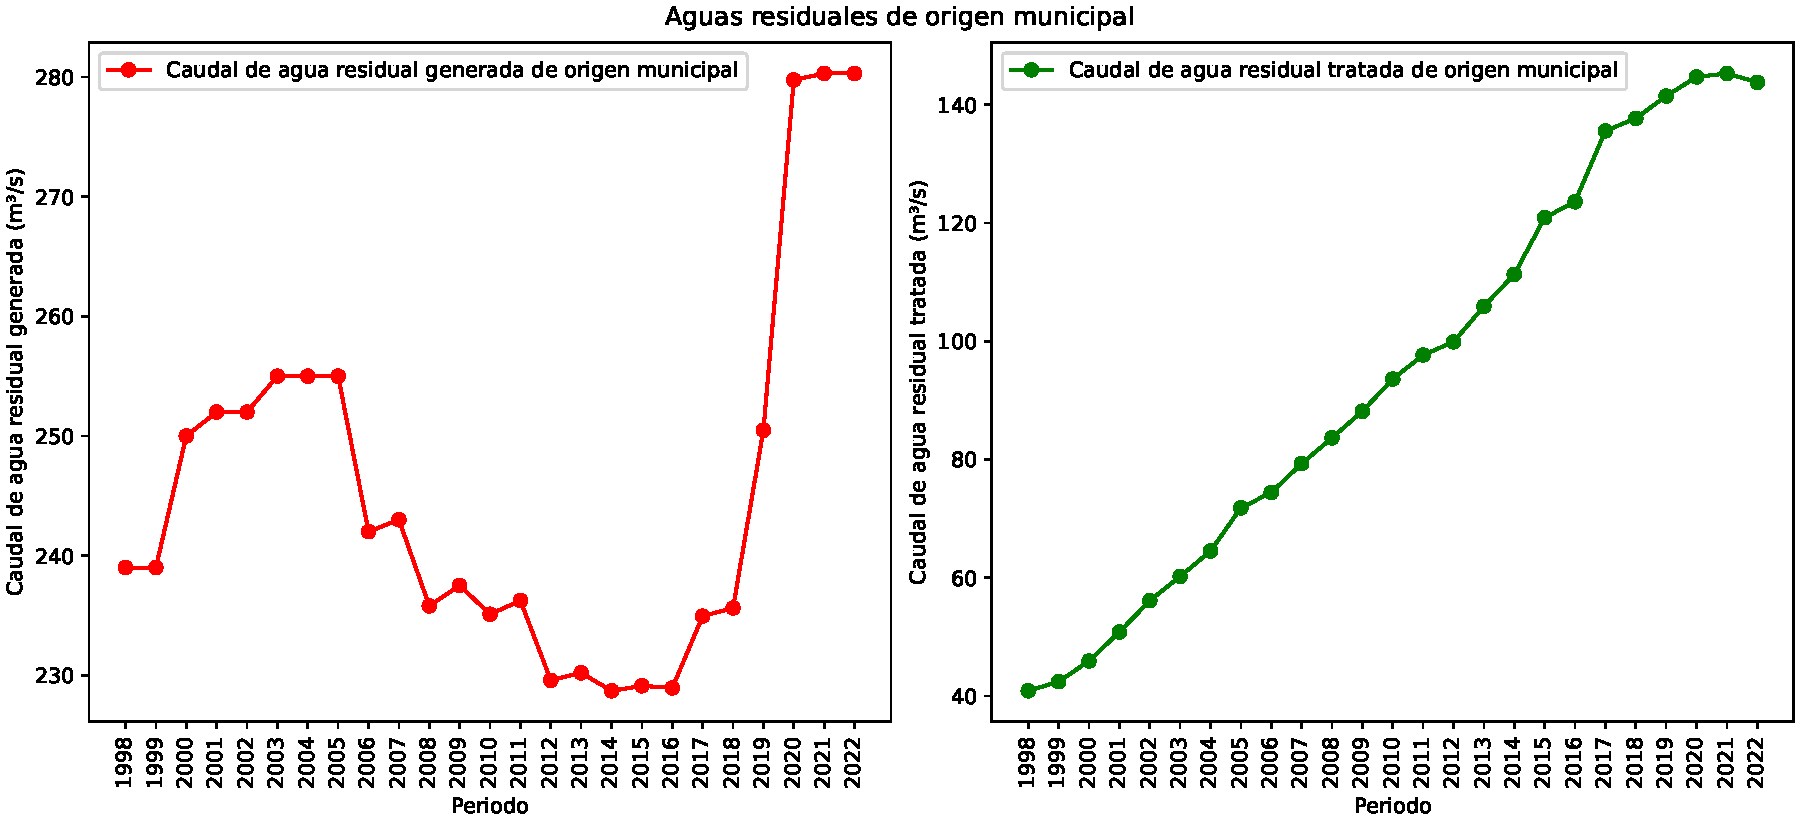
\includegraphics[scale=0.45]{../Images/AR_municipal_svg-tex.pdf}
	\\\small{Fuente: \cite{INEGIJAL}}
	\caption{Caudal de aguas residuales de tipo municipal generadas comparado al caudal de aguas que reciben algún tratamiento}
\end{figure}
\subsubsection{Aguas residuales industriales}
Este tipo de aguas provienen de las grandes industrias, a diferencia de las anteriores, estas se caracterizan por estar fuera de las zonas pobladas y debido a su alto contenido en partículas recalcitrantes, estas deben de recibir un tratamiento previo a ser vertidas a los sistemas de alcantarillado público. generalmente cuentan con un número elevado de metales pesados, pH extremo, altos niveles de materia orgánica, solventes y sustancias tóxicas~\citep{lazcano2016}.\par
La cantidad y composición de las diferentes sustancias contaminantes se ven relacionadas al tipo de proceso que se realiza, así como a la disposición que cada industria toma respecto al tratamiento de sus residuos \citep{Hanchang2009}.
\begin{figure}[H]
	\centering
	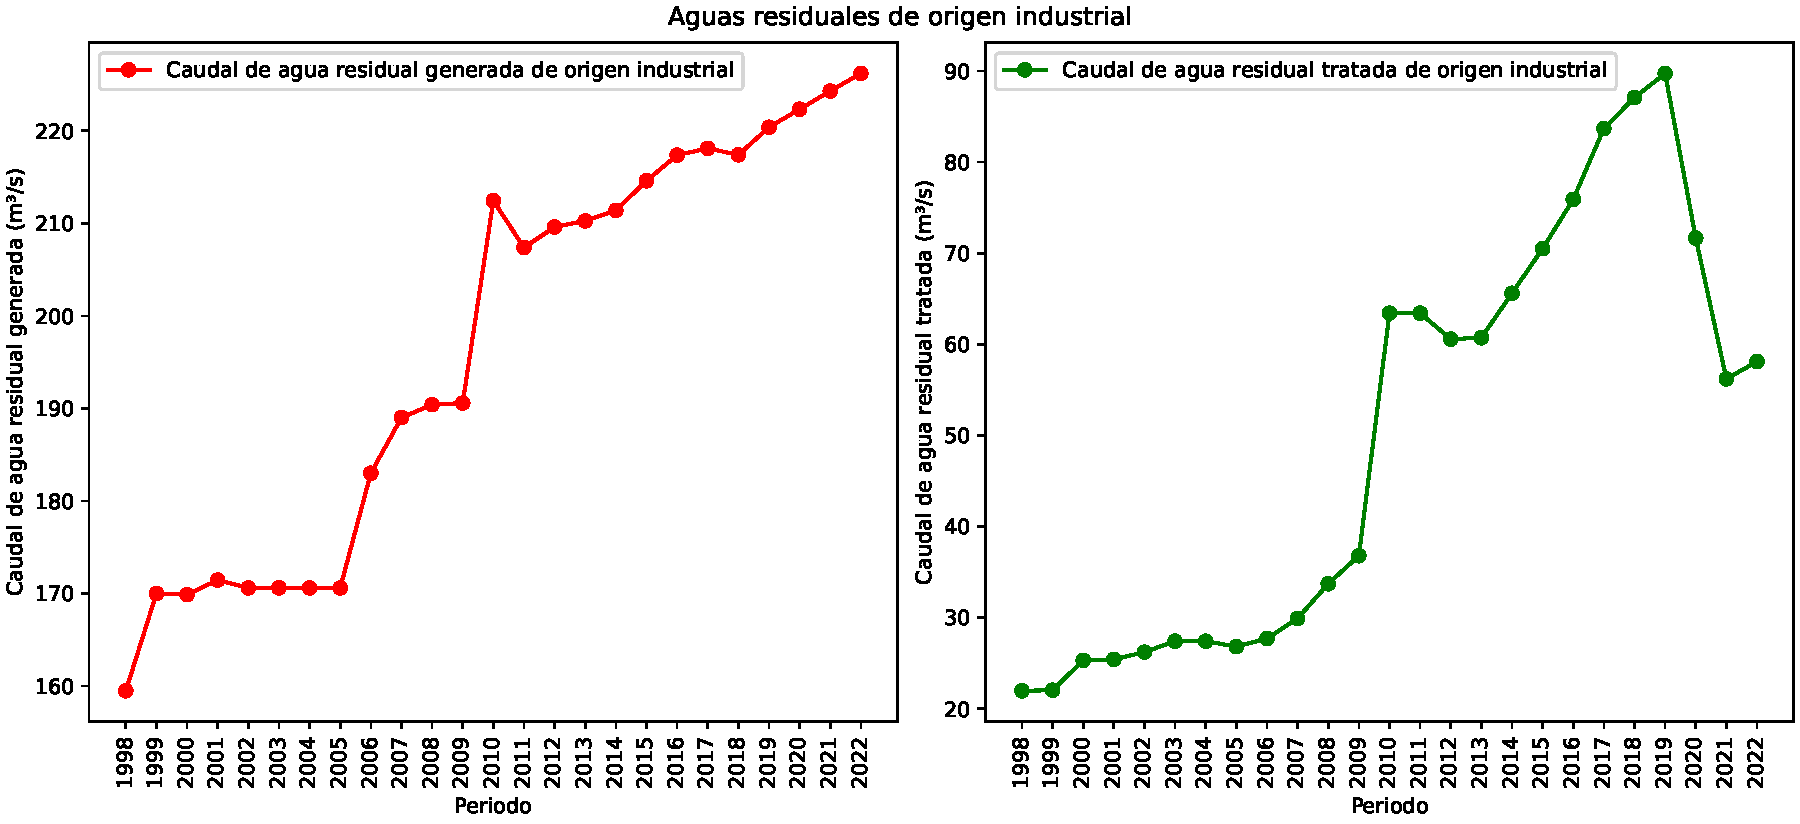
\includegraphics[scale=0.45]{../Images/AR_industrial.pdf}
	\\\small{Fuente: \cite{INEGIJAL}}
	\caption{Caudal de aguas residuales de tipo industrial generadas comparado al caudal de aguas que reciben algún tratamiento}
\end{figure}
\subsubsection{Aguas residuales agropecuarias o agroindustriales}
Son todos aquellos flujos de agua provenientes de cualquier actividad agrícola y pecuaria. Se encuentran constituidas por una gran cantidad de materia orgánica proveniente del estiércol y purines de los animales, residuos derivados del uso de pesticidas, fertilizantes y residuos farmacéuticos de uso veterinario~\citep{lazcano2016}.\par
\cite{zambrano2009} destacan que este tipo de aguas residuales difieren según la forma en la que se tiene el ganado, la forma en que son eliminados los residuos y el estado en el que se encuentran estos. Al tener al ganado disperso en libre pastoreo, el riesgo de contaminación aumenta, ya que se depende de las condiciones hidrológicas del terreno para la dispersión de las excretas del ganado, contaminando así de manera difusa la cuenca en donde se encuentra la explotación y las cuencas aledañas por medio del arrastre de los contaminantes a través de escorrentías superficiales durante el temporal de lluvias.
El tipo de residuos generados por las actividades pecuarias resultan similares a los del tipo doméstico, diferenciándose de los últimos en el volumen de agua con el que son desechados; generando como resultado directo la elevada carga de materia orgánica y sólidos en suspensión.\par
\begin{table}[H]
	\centering
	\caption{Comparación de valores obtenidos en campo con los límites máximos permisibles}
	\label{tab:Aguaagro}
	\begin{tabular}{lcc}
		\noalign{\hrule height 3pt}
		Indicador                      & Valores \emph{in-situ} & Límites máximos permisibles\tablefootnote{Según el extracto de la norma de vertimiento NC 27/1999 para ríos y embalses de Cuba} \\
		\hline
		pH                             & 7.2             & 6.5--8.5                    \\
		DBO5 (mg/L)                    & 335             & 30                          \\
		DQO (mg/L)                     & 733             & 70                          \\
		Conductividad eléctrica (S/cm) & 1100            & 1400                        \\
		Sólidos Suspendidos (mg/L)     & 10.5            & 1                           \\
		Nitrógeno total (mg/L)         & 42.9            & 5                           \\
		Fósforo total (mg/L)           & 9.17            & 2  \\ \hline      
	\end{tabular}
	\\
	\small{Fuente: }
\end{table}
\subsubsection{Aguas residuales de orígen minero-metalúrgico}
Los efluentes provenientes de la actividad minera son considerados los más tóxicos debido a su alto contenido en metales pesados como el plomo, mercurio, cadmio y zinc; ademas de metaloides antimonio y el arsénico. En países donde la mayor parte de las regulaciones son ignoradas o no son tan estrictas, la cantidad de estos elementos tóxicos supera con creces los límites máximos permitidos, dificultando aún más el tratamiento por medios convencionales. Debido a su alto número en compuestos abióticos, es necesario que este tipo de afluentes reciban un tratamiento anterior a la entrada de cualquier sistema de tratamiento biológico~\citep{lazcano2016}.
\subsubsection{Aguas pluviales}
Aquellas aguas provenientes de las precipitaciones que terminan en las alcantarillas logran disminuir la carga orgánica que hay en el desagüe, sin embargo, el cambio en las concentraciones produce variaciones en las características fisicoquímicas del agua. Otro aspecto que se debe tomar en cuenta al momento de diseñar un sistema de alcantarillado y de tratamiento es el aumento en los caudales durante el temporal de lluvia~\citep{lazcano2016}.
\subsection{Características de las aguas residuales}
El 
\subsection{Características Físicas}
\subsubsection{Sólidos}
Uno de los principales componentes físicos presentes en las aguas residuales son los materiales sólidos dispersos por todo el afluente. El tamaño de estas partículas puede variar desde cabellos hasta materiales coloidales. La clasificación de los distintos sólidos se realiza tomando en cuenta el estado y la naturaleza de los componentes de la muestra a analizar; entre los que se identifican:
\begin{enumerate}[a.]
	\item \textbf{Sólidos totales (ST)}\par
	Se definen como los residuos que quedan después de que la muestra ha sido evaporada y secada a 105 °C \unichar{"00B1} 2 °C durante 24 horas en un horno de calor seco~\citep{Economia2015}
	\item \textbf{Sólidos Sedimentables (SD)} \par
	
	\item \textbf{Sólidos Totales Volátiles (STV)} \par
	Cantidad de materia orgánica e inorgánica que se volatiliza por efecto de la calcinación a 550 °C \unichar{"00B1} 50 °C~\citep{Economia2015}.
	\item \textbf{Sólidos Disueltos Totales (SDT)} \par
	Es el material soluble constituido por materia orgánica e inorgánica que permanece como residuo después de evaporar y secar una muestra previamente filtrada a través de un filtro de fibra de vidrio con poro de 1.5 \unichar{"00B5}m a una temperatura de 105 °C \unichar{"00B1} 2 °C~\citep{Economia2015}.
	\item \textbf{Sólidos Suspendidos Totales (SST)} \par
	Es el material constituido por los sólidos sedimentables, los sólidos  suspendidos y coloidales que son retenidos por un filtro de fibra de vidrio con poro de 1.5 \unichar{"00B5}m secado y llevado a masa constante a una temperatura de 105 °C \unichar{"00B1} 2 °C~\citep{Economia2015}.
	\item \textbf{Sólidos Suspendidos Volátiles (SSV)} \par                
	Son aquellos sólidos suspendidos que se volatilizan en la calcinación a 550 °C \unichar{"00B1} 50 °C~\citep{Economia2015}.
\end{enumerate}
\subsubsection{Temperatura}
\subsubsection{Color}
\subsubsection{Olor}
\subsection{Características Químicas}
\subsubsection{Orgánicos}
\begin{enumerate}[a.]
	\item 
\end{enumerate}
\subsubsection{Inorgánicos}
\begin{enumerate}[a.]
	\item 
\end{enumerate}
\subsubsection{Gases}
\begin{enumerate}[a.]
	\item 
\end{enumerate}
\subsection{Características Biológicas}
\subsection{Muestreo}
\subsection{Límites máximos permisibles}\label{NOM2021}
\subsection{Tratamiento de aguas residuales}

\subsubsection{Tratamientos biológicos}
El uso de organismos vivos con el fin de reducir la cantidad de materia orgánica presente en las aguas negras se remonta a finales del siglo XIX y principios del XX en Inglaterra como resultado de varias observaciones en las denominadas \emph{granjas de aguas negras}, en donde las aguas negras provenientes de las urbanizaciones eran filtradas por medio de filtros de arena, escombros, pizarra, ladrillos, entro otros materiales pétreos porosos. Gracias a las características de estos lechos, pronto permitieron el crecimiento de varias comunidades microbianas capaces de alimentarse de la materia orgánica disuelta en las aguas residuales, reduciendo el número de contaminantes a niveles más aceptables~\citep{Fair2008}\par
A consecuencia de el desarrollo de las grandes ciudades, el uso de sistemas biológicos fue adquiriendo más usos a parte de la remoción de materia orgánica. Entre estos nuevos usos se destacan la nitrificación de aguas con alto contenido de nitrógeno amoniacal, la desnitrificación 
\subsubsection{Procesos biológicos de cultivo en suspensión}
\subsubsection{Procesos biológicos de soporte sólido}
\subsection{Lodos Activados}
Dentro de los procesos basados en cultivo de microorganismos en suspensión, uno de los más importantes, y a su vez mas utilizados, es el que involucra la utilización de lodos activados como agentes reductores de la carga orgánica presente en el afluente a tratar.
\subsubsection{Flóculos}
\subsubsection{Bulking filamentoso}
\subsection{Modelos matemáticos en el proceso de lodos activados}
\subsubsection{Modelo de Monod}
\subsubsection{Modelo de Arrhenius}
\subsection{Planta tratadora de aguas residuales municipal de Lagos de Moreno}
\subsection{MATLAB®}
